\documentclass[tikz]{standalone}

\usepackage{amsmath}
\usepackage{lmodern}
\usepackage{pgfplots}
\usepackage{physics}

\pgfplotsset{compat=1.17}

\definecolor{exotic orange}{RGB}{255,128,0}
\definecolor{exotic green}{RGB}{0,102,102}
\definecolor{exotic blue}{RGB}{0,202,161}
\definecolor{exotic red}{RGB}{250,86,86}

\begin{document}
	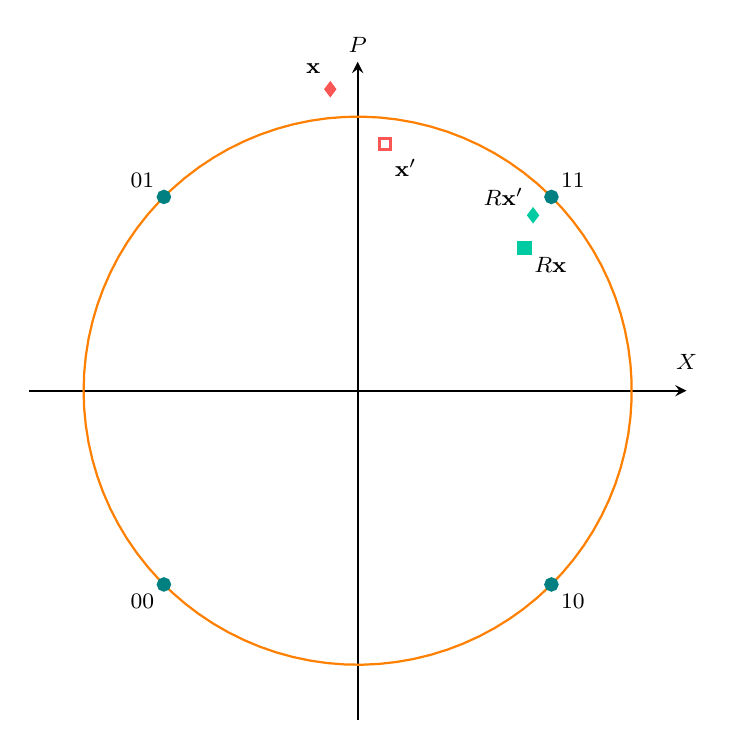
\begin{tikzpicture}[
		font=\fontsize{8}{9}\selectfont,
	]
		\begin{axis}[
			width=0.95\linewidth,
			axis lines=center,
			axis equal image,
			xlabel={$X$},
			ylabel={$P$},
			ticks=none,
			xmin=-1.2,
			xmax=+1.2,
			ymin=-1.2,
			ymax=+1.2,
			domain=-180:180,
			samples=100,
			axis line style={thick},
			x label style={
				at={(axis description cs:1,0.57)},
				anchor=north,
			},
			y label style={
				at={(axis description cs:0.5,1)},
				anchor=south,
			},
			cycle list name=exotic,
			every mark/.append style={solid},
		]
			\addplot+[very thick, only marks] coordinates {(0.707,0.707) (0.707,-0.707) (-0.707,0.707)(-0.707,-0.707)};
			\node[above right] at (axis cs:0.707,0.707) {$11$};
			\node[below right] at (axis cs:0.707,-0.707) {$10$};
			\node[below left] at (axis cs:-0.707,-0.707) {$00$};
			\node[above left] at (axis cs:-0.707,0.707) {$01$};	
			\addplot+[thick, no markers] ({cos(x)},{sin(x)});
			
			\addplot+[very thick, mark=square, exotic red] coordinates {(0.1,0.9)};
			\addplot+[very thick, mark=diamond*, exotic red] coordinates {(-0.1,1.1)};
			\node[above left, yshift=2] at (axis cs:-0.1,1.1) {$\vb{x}$};
			\node[below right, yshift=-2] at (axis cs:0.1,0.9) {$\vb{x}^\prime$};
			
			\addplot+[very thick, only marks, mark=diamond*, exotic blue] coordinates {(0.64,0.64)};
			\node[above left] at (axis cs:0.64,0.64) {$R\vb{x}^\prime$};
			\addplot[very thick, only marks, mark=square*, exotic blue] coordinates {(0.609,0.521)};
			\node[below right] at (axis cs:0.609,0.521) {$R\vb{x}$};
		\end{axis}
	\end{tikzpicture}
\end{document}